\subsection{Tests}
As the models are best understood visually by looking at the graphs produced, any failsafe way to ensure that every run produces meaningful results can be hard.
However, there are expected values for cases where only $a$, $b$ and $c$ are considered, in which the results can be compared to.
Additionally, comparing the RK ODE solver's results with the MC solver's results can give some indication as to whether the program is working, given that these independent methods produce the same results.


\subsubsection{Testing the RK solver with expected values}
As the MC solver has quite a bit of variance after reaching the steady state, a numeric test for the RK solver is more feasable.
By requiring that the final value for lets say $I$ is equal to the expected value within some error $\epsilon$, we can test against the expected values.
The expected values are also plotted as horizontal dashed lines when the total population is static as seen in \textit{Figure} \ref{fig:comparetest}.

\begin{figure}[]
    \centering
    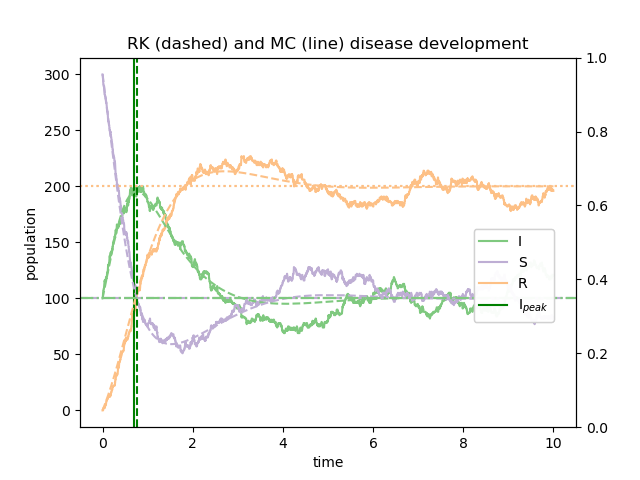
\includegraphics[scale=0.55]{plots/Compare_getstd_a_4_b_1_c_0.5.png}
    \caption{Comparison of RK solver (dashed) and MC simulation (line) with expected values (horizontal dashed) with $a=4$, $b=1$ and $c=0.5$}
    \label{fig:comparetest}
\end{figure}

\subsubsection{Testing the population manager in the MC solver}
As mentioned already, due to the variance in the MC solver, comparing its final state to some expected value isn't really feasable.
Therefore, unit tests are checking that the population manager, which ads, removes and manages the states of members of the population, is funcitoning properly.
With this unit test passed, and with visual comparison of the RK solver and the MC simulations' plots, results are more trustworthy.



\subsection{Optimizations and runtimes}
While the RK solver is an algorithm already developed by others, it can't really be optimized much, as it can't run in paralell processes, or simplified much more,
the MC solver probably can be optimized a lot. Every person in the population has a lot of if statements to check if the RNG is within the transition probabilities.
I am not familiar of any other way to check for RNG<P, and as such if statements are significantly slowing down the simulations.

\begin{table}
    \centering 
    \begin{tabular}{l|c|c|c}
        Method & MC Cycles/steps & Population & Runtime \\
        \hline
        RK (2EQ) & 2399 & 400 & 0.00015s \\
        RK (3EQ)   &2399 &400 & 0.00018s \\
        RK (2EQ) & 100000 & 400 & 0.0069s \\
        RK (3EQ) & 100000 & 400 & 0.0072s \\
        MC (no OpenMP) & 2399 & 400 & 0.083s \\
        MC (OpenMP) & 2399 & 400 & 0.31s
    \end{tabular}
    \caption{A comparison of runtimes between the RK solver and the MC solver.}
    \label{tab:single_runtimes}
\end{table}

In \textit{Table} \ref{tab:single_runtimes}, the RK solver is significantly faster than the MC solver.
Simplifying from 3 equations to 2 in the RK solver also seems to reduce runtimes somewhat, but not signifficantly.
This is likely due to the MC solver doing logic on every single member of the population, while the RK solver calculates the whole population at once.
To speed this up, it was attempted to implement OpenMP on the cycle throught the population in the MC solver, however it seemed to create silly results and run slower, so this was not attempted to implement properly.


\subsubsection{2 vs 3 equations in RK solver}
As metioned briefly already, in order to speed up the RK solver a bit, it checks whether it can simplify from 3 to 2 equatins.
When the population is stable, such that $N$ is constant, we have that
\begin{equation}
    N=I+R+S
\end{equation}
Which can be simplified such that
$$
R=N-R-S
$$
So that $R$ is plugged into the equation for $S$, and we only need 2 equations. 
However, as is the case with the vital parameters where N is changing, we now have to update N and R, which depend on each other, 
which is no longer possible. This version of the RK-model turns out to be slightly slower, as R now needs to be calculated for every step.


\subsubsection{Using array of functions to avoid if-statements in MC solver}
Like described already, different inputs leads to different transitions being evaluated in the MC solver. 
In an effort to reduce the amount of if-statements, the pointers to the relevant transition functions evaluating a potential state change are put in an array.
In the array, there is one function per state, and as such, the integer representing the state of the currently evaluated member of the population is used to index the array to call the corresponding function. 
As such, only the get state function which returns an integer is called from the Person class, and an if-statement is avoided.

\subsubsection{Compiler flag optimizations}
To further increase performance of the program, OpenMP is implemented for consecutive runs of the MC simulation, used to gather statistics 
for the time of infection peak and when zero infections is reached. Additionally compiler flag optimization -O is compared to -O3.
In \textit{Table} \ref{tab:compilerflags}, we see signifficant performance increase in both MC and RK for -O3, and for OpenMP in MC.

\begin{table}[!h]
    \centering
    \begin{tabular}{l|c|c|c|c|c}
        Method & Optimizations & MC Cycles/steps & Consecutive runs &Population & Runtime \\
        \hline
        RK & None & 10 000 & 1 &400 & 0.0018s \\
        RK & -O3 & 10 000 & 1 &400 & 0.00083s \\

        MC & None &2399 & 20 & 400 & 17.83s \\
        MC & -O3 &2399 & 20 & 400 & 1.65s \\
        MC & -O3 OpenMP&2399 & 20 & 400 & 0.38s \\
    \end{tabular}
    \caption{Runtimes with different compiler flag opimizations for single run RK and multiple run MC.}
    \label{tab:compilerflags}
\end{table}